\documentclass[]{article}
\usepackage{pdfpages}
\usepackage[toc,page]{appendix}
\usepackage[toc,section=section]{glossaries}
\usepackage{imakeidx}
\usepackage{biblatex}
\usepackage{graphicx}
\usepackage{float}
\usepackage{listings}
\usepackage{selinput}
\usepackage{changepage}

\addbibresource{bib.bib}

\makeglossaries{}
\loadglsentries{entries}
\makeindex

\nocite{*}

\title{Fennel Protocol: An Identity-Aware Signal Layer\\\large{Revision 3}}
\author{Sean Batzel, Mateusz Plaza, Andrew Plaza}

\begin{document}

\maketitle
\begin{abstract}
Fennel Protocol began as a Web of Trust mechanism allowing signals to propagate through communities developed by the members of those communities. This has expanded in the subsequent months, with the concept growing to encompass a number of further use cases, outlined in this document. The protocol itself shall be implemented as a self-contained blockchain constructed using the Substrate framework, promoting a focus on blockchain-to-blockchain communication and interoperability. Fennel Protocol itself will revolve around transaction-based signature-certified attestation events, used for permission controls, supply chain tracing, and an expanding number of use cases. This document shall act as a general outline of the Protocol and as a technical supplement to the main proposal for each of these use cases.
\end{abstract}
\clearpage

\tableofcontents

\listoffigures
\listoftables
\clearpage

\section{The Root of Digital Identity on Fennel}
\label{scrivauto:10}

Fennel Protocol's major features will include a focus on extensible, interoperable, modular digital identities. While other protocols exist that provide identities, Fennel Protocol will provide a bridge between those protocols and its own concept of digital decentralized identity. This interoperability will enable powerful applications of transactional identity management, starting with a series of features baked in to the Fennel Protocol node software itself.

\subsection{The Identity Transaction}
\label{scrivauto:11}

Every top-level identification event occurs as a transaction on the Fennel Blockchain. When an individual or organization announces themselves to the Protocol, a new transaction with identifying information (including, in the case that the identity is for and individual or group, application-specific public keys) is broadcast to the network. This is termed the Create transaction, and is the starting point for every personal, group, or object identity managed by Fennel Protocol. Through a chain of transactions pointing to the original one, we can create an \textit{identity certificate}. This functions similarly to an NFT - it is a group of transactions, unique to the person or object that it refers to and unique amongst all other identity certificates. However, unlike NFTs, this is intended to form the root of an actor's entire presence on Fennel Protocol.
The goal of this transaction structure is to expand the existing identity pallet's functionality to encompass updates. Currently any time a verified identity needs to be changed it needs to be entirely reissued and verified again. Under Fennel Protocol, individual features of a modular identity may be verified, so if an update is committed to an identity an application may easily display what has changed, what elements are verified, and what elements are unverified. Verification of identities and identity elements will occur through the Sign transaction, similar to signing the identity's public key.

\subsection{Managing Certification}
\label{scrivauto:12}

As mentioned before, every certificate on Fennel Protocol is no more than a collection (a ``chain'') of transactions tracing the history of an identity or asset. This aggregated identity is used as the focal point of every application on Fennel Protocol, as will be discussed in following pages. This is all done with efficiency in mind, based on an understanding that an aggregation of small adjustments will be simpler to manage on a macro scale than a sprawling identity concept with extremely large payloads in each transaction.

We define three fundamental operations on every certificate chain - a Creation operation, an Update operation, and a Revoke operation which are called by the initial owner of the identity, be it an asset or personal identity. We also define a Sign operation callable by other members of the network to issue a transaction attesting that the target identity is trusted and/or verified by the identity issuing the signature. The Sign operation will also be instrumental in operations giving access permissions or transferring asset ownership.

\section{Using Fennel to Form Actor-to-Actor Networks}
\label{scrivauto:13}

The main functions of Fennel Protocol lie in a focus on decentralized actor-to-actor networks, whether the actors are applications, machines, or end users. In fact, Fennel Protocol is named for the nodular structure of the Fennel plant, which strongly resembles a graph diagram like the kind we expect to see out of the graphs modeled by the Protocol.

\subsection{Identity Interplay}
\label{scrivauto:14}

Almost every major Fennel Protocol feature relies on interactions between identity transactions. In this subsection, we'll expand on the previously-mentioned Sign operation and what expanded operations can be defined on it as a baseline.

\subsubsection{Motivating Identity Interactions}
\label{scrivauto:15}

As discussed previously, Fennel Protocol's main features are centered around the way that individuals and applications interact with clearly-identified entities. Since we're building on a custom blockchain, the simplest and most effective manner of transmitting information between identities is in compounding transactions. This means that anyone on Fennel Protocol can create a series of messages that acts as its own history of actions, validated by their presence on the chain. These messages can then be used to generate an aggregated picture of the state of the identity represented by the account making these transactions. In the next subsection, we'll discuss the way that these messages can be conceptualized and secured.
The chain of compounding transactions will rely on off-chain compilation to generate a result identity. On-chain computation will be limited, so all that is needed is a transaction pointing to the identity and the last transaction updating that identity. As applications receive transactions from the network, they will use the contents of the transactions to recreate the chain's identities in their own data context. This will allow management of identities with as little performance overhead as possible on the protocol's end.
Identity transactions will enable authentication between apps and between individuals by maintaining a decentralized, modular, updatable concept of identity.

\subsubsection{Transactions as Messages}
\label{scrivauto:16}

The transactional nature of every action taken on Fennel Protocol means that messages with less sensitive content can be broadcast to identities known to the chain. These messages should be expiring, sent as a transaction specifying recipient, sender, and content, and either encrypted for a group or public. Sealed sender is a strong possibility in cases where the parties are known to one another prior to transmission of the transaction. Since the architecture of Fennel Protocol is designed with rapid consensus in mind, these messages immediately have the capacity to become instrumental to organizing operations between nodes in the network. As a result, these transactional messages leverage the blockchain in a manner very similar to that in which the messages you might see in a network-oriented protocol use the underlying transport layers. This leads to very clean decentralization - rather than needing to identify each peer and transmit messages to it, an application can choose to allow access to any application implementing its unique interface on Fennel Protocol.

\subsection{Network Features}
\label{scrivauto:17}

The protocol itself enables a number of features for producing immutable, secure, provable connections between parties. This extends to creating logical social and application networks that can be leveraged to power extremely complex dynamics.

\subsubsection{Application-Configurable Webs of Trust}
\label{scrivauto:18}

One of the earliest strengths of Fennel Protocol was a capacity to construct simple webs of trust based on transactions attesting to the trustworthiness of other actors on the network. This functionality will be highly parameterized and customizable by each application, but the process will be identical across applications and experiences.
Fennel Protocol will achieve the creation of these Webs of Trust through the same mechanism that certification applications will use - the Sign operation. These will directly represent edges connecting the nodes of the Web, leading to extremely lightweight on-chain representation and therefore fairly simple consensus on trust actions. This modified Sign operation will indicate what it is - a Trust transaction - and provide either a GRANT command with a 1-5 integer argument representing the level of trust, or a REVOKE command.

\subsubsection{Three-Way Handshake}
\label{scrivauto:19}

The three-way handshake discussed will occur similarly to the standard three-way handshake involved in HTTPS. An asymmetric encryption channel will be established between two parties by using their Fennel-hosted public keys. Eventually the protocol will be expanded to support many, if not most, popular public-key encryption methods, though RSA will be used in early versions. Key negotiation will occur by generating two individual shared secrets and generating a derivative shared encryption key.
Crucially, these symmetric keys will expire fairly rapidly. This will require frequent reconnections to reestablish known secure shared secrets.

\subsubsection{Establishing Encrypted Channels}
\label{scrivauto:20}

By projecting public keys to the network, we provide users with a simple way to send encrypted messages to one another. The three-way handshake process (or the Diffie-Hellman process, in some cases) will be discussed on several occasions throughout this document. By establishing a secure connection through this multi-way handshake, information can be secured fairly quickly. From there the protocol will expose endpoints for applications to use to carry out interactions, similar to an encrypted phone line, or a standardized process by which applications can identify each other directly by public IP address and establish traditional TCP/IP interactions. This will likely be used more by applications designed by third parties to interact with one another.

\section{Fennel in a Distributed Computing Setting}
\label{scrivauto:21}

Fennel Protocol will enable nodes in decentralized computing applications with a number of unrelated owners to interact clearly with one another behind encrypted channels. To keep consensus moving smoothly, we'll want to offload a good deal of heavy lifting to off-chain workers or the endpoint applications themselves. The latter task will be handled through the aforementioned safe IP address exposure process.

\subsection{IP Address Obfuscation}
\label{scrivauto:22}

In order to protect the nodes participating in operations on Fennel Protocol from public exposure, we need a way to protect IP addresses (or any other short piece of identifying information, for that matter). The simplest way to do this is by establishing an encrypted channel between two endpoints - in this case, often two machines participating in a Fennel Protocol application. By using one of the off-chain message channels, applications will be capable of exchanging their machines' IP addresses in a manner that is both transient and encrypted, leading to far less sensitive information about endpoints being leaked than if the exchange occurred on-chain.\footnote{In the first version of this document, we will leave out whether this is done through a parallel server or through an off-chain worker. Further work is needed to determine which is most effective.}

\subsection{Node Orchestration in Distributed Data Networks}
\label{scrivauto:23}

By building on the features we've mentioned so far, we can expand to a set of further functionalities which will allow machines participating in decentralized applications to directly interact with one another to carry out application-critical exchanges. This will occur most often ``in the wild'' as data access permission management. The owner of one node will issue a Sign transaction to the owner of another node specifying (in a manner specific to the application) what particular resources that identity has access to.\footnote{An example of this is given in Team fEMR: Identity Certificates as a Permission Management Scheme.}

\section{Interacting with Fennel Protocol}
\label{scrivauto:24}

Like most blockchains, Fennel Protocol will expose its functionalities to other applications through Remote Procedure Calls. These will be somewhat complex, as Fennel Protocol is built with the intention of being a highly extensible protocol. 

\subsection{Fennel Extrinsics}
\label{scrivauto:25}

With the goal of allowing interprocess communication we'll begin to define the extrinsics on Fennel Protocol. These will be callable through the standard Substrate JSON RPC that applications may use to directly interact with Fennel Protocol. Any action taken on this RPC will require a valid identity and signed operations to create a transaction, as with all blockchain RPCs. The procedures available will be split into two categories - Base Operations and Extended Operations.

\subsection{Base Operations}
\label{scrivauto:26}

Base operations include the first four functions exposed by the Protocol - Create, Update, Sign, and Revoke. These are extremely small payloads transmitted as transactions between two accounts.
It is important to note that Fennel Protocol will allow highly flexible use of these operations. Any identity on-chain is a valid target for any of these operations, allowing applications to track transactions connecting individuals to the applications themselves, transactions connecting individuals to themselves, or transactions connecting individuals to each other. 

\subsection{Extended Operations}
\label{scrivauto:27}

Extended operations are modified versions of the Sign operation. The difference is in optional payload modifiers attached to the content of the RPC call.
We shall use the Web of Trust application as an example for how this will work. In this case, the Sign operation is still a signed transaction linking two accounts together, but will be designated a TRUST transaction and enhanced with a RATING field. It should be fairly trivial to see where this RATING field can be leveraged in other applications. TRUST transactions will be interpreted by applications utilizing them as edges connecting accounts, represented in a standard network graph as vertices. From her webs can be constructed and interpreted quite easily as the end user needs - rating functions can be defined in endpoint software, essentially offloading any interpretation of the Web of Trust away from Fennel Protocol and reducing the concern for slowed consensus.

\section{Fennel Token}
\label{scrivauto:28}

The core governance and validation asset of Fennel Protocol will be the Fennel Token. The Token shall be expected to carry some value, but this value will work toward incentivizing honest behavior on the network. We have a current set of three expected use cases that will directly utilize the Token.

\subsection{Transaction Fees}
\label{scrivauto:29}

Similar to the manner in which other blockchains generally incentivize miners to validate the integrity of the network, Fennel Protocol will rely on small transaction fees paid to the network to provide its validators and users with inventives to participate in the overall economy of the network. The exact price will be up to the economy model defined in the Substrate construction of the blockchain.

\subsection{Monetized Risk-Based Certification}
\label{scrivauto:30}

One of the major use cases for Fennel Token will be as an attestation network incentive. Participants in any network will have a natural inclination to make more accurate judgements if they have an immediate stake to lose. A very small volume of Tokens will be required as a lock on every Sign operation, and will be considered at risk in the event that the attested identity is found to have acted against the conditions of their behavior in the network.

\subsection{Monetized Data Retrieval}
\label{scrivauto:31}

By connecting data to identity and tracing provenance, we can create means for individuals to monetize their own data. This feature will tie in with permission management and access control, but will not always be involved. In this case we shall implement a tag on an on-chain, data-connected identity requiring a specialized Sign transaction from the individual \textit{requesting }access to the contents of the identity. The recipient will designate the identity as either one that requires a returned Sign transaction \textit{granting }access, or one that requires a certain volume of Fennel Token to be attached to the value of the incoming request to unlock the data.\footnote{This process will be functionally quite similar to the process of unlocking content when an NFT is purchased.}

\section{Use Case Explorations}
\label{scrivauto:32}

Fennel Protocol evolved out of a set of core use cases that needed a common featureset to address their unique needs. This subsection will outline the manner in which these will directly leverage the architecture of Fennel Protocol.

\subsection{Team fEMR: Identity Certificates as a Permission Management Scheme}
\label{scrivauto:33}

Team fEMR's application use case will use the aforementioned node orchestration scheme to create secure, encrypted channels between nodes. Every candidate node of the fEMR On-Chain network will create, of course, an identity for itself. This will occur whether the node is an official one rolled out by Team fEMR or an unofficial one attempting to be verified as a supported deployment.

\subsubsection{Permission Control}
\label{scrivauto:34}

The same certification method described above will allow applications to assign permissions to identities. The above node structure will require an official Team fEMR account on Fennel Protocol to execute a Sign call pointed toward the identity of any node requesting to enter the fEMR On-Chain network. This can be either unprompted or from a ``request''-designated Sign call sent from the requesting entity to fEMR.

\subsubsection{Node Orchestration}
\label{scrivauto:35}

In this subsection, we'll describe a concrete example of the system proposed in our discussion of Fennel Protocol's applications in Distributed Computing. Identities certified by the main Team fEMR account may participate in the encrypted channel creation process and the node connection orchestration process, thereby forming a double-secured conduit for fEMR On-Chain data to pass peer-to-peer through another secure medium. The fEMR On-Chain software itself will expose an API layer 

\subsubsection{Data Interchange}
\label{scrivauto:36}

Encrypted channels created by Fennel Protocol are a perfect opportunity for clean, secure data interchange between nodes running common software. Two installations of fEMR OnChain will be capable of exchanging data with very low risk of leak.
Prior to transmission between nodes, fEMR's use case will leverage blockchain-based signatures on every patient interaction to prove the transaction has been placed by a trusted party. In parallel to QLDB, each node's local database will store a record consisting of a pointer to the updated data and a Fennel signature on the JSON payload generated by that update. Functions will be integrated into OnChain's backend providing fast verification and traceability of signed transactions, as well as a signal mechanism that will alert a Campaign's manager if an invalid or untrusted signature is detected.

\subsection{Supply Chain Counterfeiting Resistance: Identity-Rooted Provenance Chains}
\label{scrivauto:37}

Supply chain management can be seen as just another network of interacting identities - a set of identities for the individuals acquiring assets, and identities for the assets themselves. Essentially these asset identities can be seen as evolving NFTs without a strictly connected value.

\subsubsection{Certification of Physical Objects}
\label{scrivauto:38}

Representation of physical objects is in no way new territory to blockchains - NFTs have existed for several years and allow for tokenization of just about any object or concept. We'll create a similar effect through a transaction creating a new identity (this time without an encryption keypair) that identifies itself as the item in question. This identity then becomes the subject of Sign operations indicating that the item has changed hands, or Update operations adding new attributes or information to the identity in question.

\subsubsection{Transactions Representing Movement of Ownership}
\label{scrivauto:39}

Similarly to the use of compounding transactions to modify characteristics of an identity, we can use compounding transactions to trace the ownership and movement of tokenized assets over time. A physical onject identity, once created, can be moved to another account through a Sign transaction carrying a signal to transfer an identity at a certain transaction ID, which creates a traceable route of the object's movement from recipient to recipient.

\subsection{WhiteFlag Protocol: Fennel Protocol as a Source of Resistance to Interception}
\label{scrivauto:40}

The WhiteFlag use case is less focused on distributed computing tasks, and more concerned with creating secure channels between identities on Fennel Protocol. This application will be largely similar to the fEMR application without the use of node orchestration features.

\subsubsection{Encrypted Channel Establishment}
\label{scrivauto:41}

WhiteFlag specifically has a strong need for secure message transmission that can be made resistant to interference from negative actors. Channels need to be established that can be effectively collapsed once they've become obsolete, but can still be referenced as evidence of a certain exchange occurring. The current implementation of WhiteFlag uses Diffie-Hellman key negotiation between identities in order to create a session-unique key. This will be available, though Fennel Protocol's default channel establishment feature will use a three-way handshake based on the public keys created by identities.

\subsubsection{Message Transmission}
\label{scrivauto:42}

When considering peer-to-peer messages on a blockchain we find an interesting challenge that doesn't appear often anywhere else - the messages transmitted are public and immutable. Even accounting for encryption of every message, if a key leaks or is in some way compromised any message ever committed to the chain can easily be retrieved and decrypted.

\section{Fennel Protocol Milestones}
\label{scrivauto:43}

The Fennel Protocol project will occur in its first iteration over three milestones, expected to take a month each.

\subsection{Certification Dynamics}
\label{scrivauto:44}

Our initial milestone will involve the creation of transaction types that allow for formation and mutation of on-chain identities. Identity mechanisms for web3 already exist - Fennel Protocol won't try to reinvent wheels that don't need reinventing. 

\subsubsection{Identity Creation}
\label{scrivauto:45}

In order for an identity to be created, whether it be for a person, an asset, or an organization, a transaction must be created which carries the basic information required to initialize the identity.

\subsubsection{Identity Mutation}
\label{scrivauto:46}

Identities on Fennel Protocol will be updated and managed through transactional state mutations. This feature will be implemented through an RPC call which retrieves the set of transactions classified as mutations to the given identity. 

\subsubsection{Identity Revocation}
\label{scrivauto:47}

Identity revocation is a serious point - if any asset or resource attached to an identity is compromised or discarded, we need a way to ensure that it is publicly declared revoked so that hijacks and issues are less likely. This will appear on-chain as a simple transaction bearing the REVOKE command, as well as the address of the original transaction's issuer and the ID of that transaction. From there, applications indexing the chain will consider the actions of that transaction invalidated.

\subsubsection{Identity Attestation Signature}
\label{scrivauto:48}

Once identities are established, we need a way for webs of trust to form between them. We've defined a Sign operation which issues a signed transaction connecting an actor to another actor. In order to create a web of trust, we'll subclass the Sign operation to create a Trust operation and a Revoke Trust operation.

\subsection{Key and Encryption Mechanisms}
\label{scrivauto:49}

Beyond its certification and identity management features, Fennel Protocol will also provide mechanisms for establishing encrypted channels of communication between participants. These will involved the blockchain slightly less, as encrypted information should really not be submitted to an immutable public record.

\subsubsection{Public Key Retrieval}
\label{scrivauto:50}

Public key retrieval is the core of the encrypted channel handshake on Fennel Protocol. Fennel nodes will expose a series of simplified query mechanisms that will allow for retrieving a public key fingerprint if an account address is needed. An off-chain storage mechanism will be used for storing and serving public keys, and will listen for fingerprint requests from participants searching for peers' public keys.

\subsubsection{Encrypted Fennel Communication Channel Negotiation}
\label{scrivauto:51}

Channel negotiation will occur in a neutral location (most often hosted by the nodes running the blockchain network) using public keys to transmit private messages. An off-chain message server (either an off-chain worker or a separate server) will be used to create initial channels between peers, similar to a standard encrypted messaging application. The first message will be an encrypted key negotiation so that a hidden shared secret can be used as a secondary layer of security.
This will, of course, require that peers that may need to interact with one another are using the same version of Fennel Protocol and the same version of the software responsible for transmitting messages to ensure parity in message format.

\subsection{Peer Detection and IP Obfuscation}
\label{scrivauto:52}

Fennel Protocol's channel negotiation mechanism will be directly used for orchestrating interactions between two peers that need to cooperate on a task. The most involved part of this will, as mentioned before, be the initial process of locating the desired peer and establishing an encrypted conduit to it.

\subsubsection{Peer Retrieval}
\label{scrivauto:53}

Peer retrieval is done through combing the chain for identities of other nodes of the distributed application searching for peers. This will likely benefit from use of the Substrate archive node, though most use cases will likely want to compile their own query-friendly records at the application level. This can be done (and will be done by several official Fennel Labs use cases) by querying new transactions periodically and updating a local database to reflect recent changes relevant to the application in question.

\subsubsection{Using Encrypted Channels to Retrieve IP Information}
\label{scrivauto:54}

The previous few subsections work together to form the root of peer-to-peer computing on Fennel Protocol - identity-aware, protected channels for exchanging sensitive orchestration and collaboration information. IP addresses will be exchanged by creating a secured Fennel Communication Channel with a Retrieved Peer and transmitting the local machine's IP address and relevant software information (such as versions or channel configuration variables).

\section{Figures}
\label{scrivauto:57}

\pagebreak
\begin{figure}[htbp]
\centering
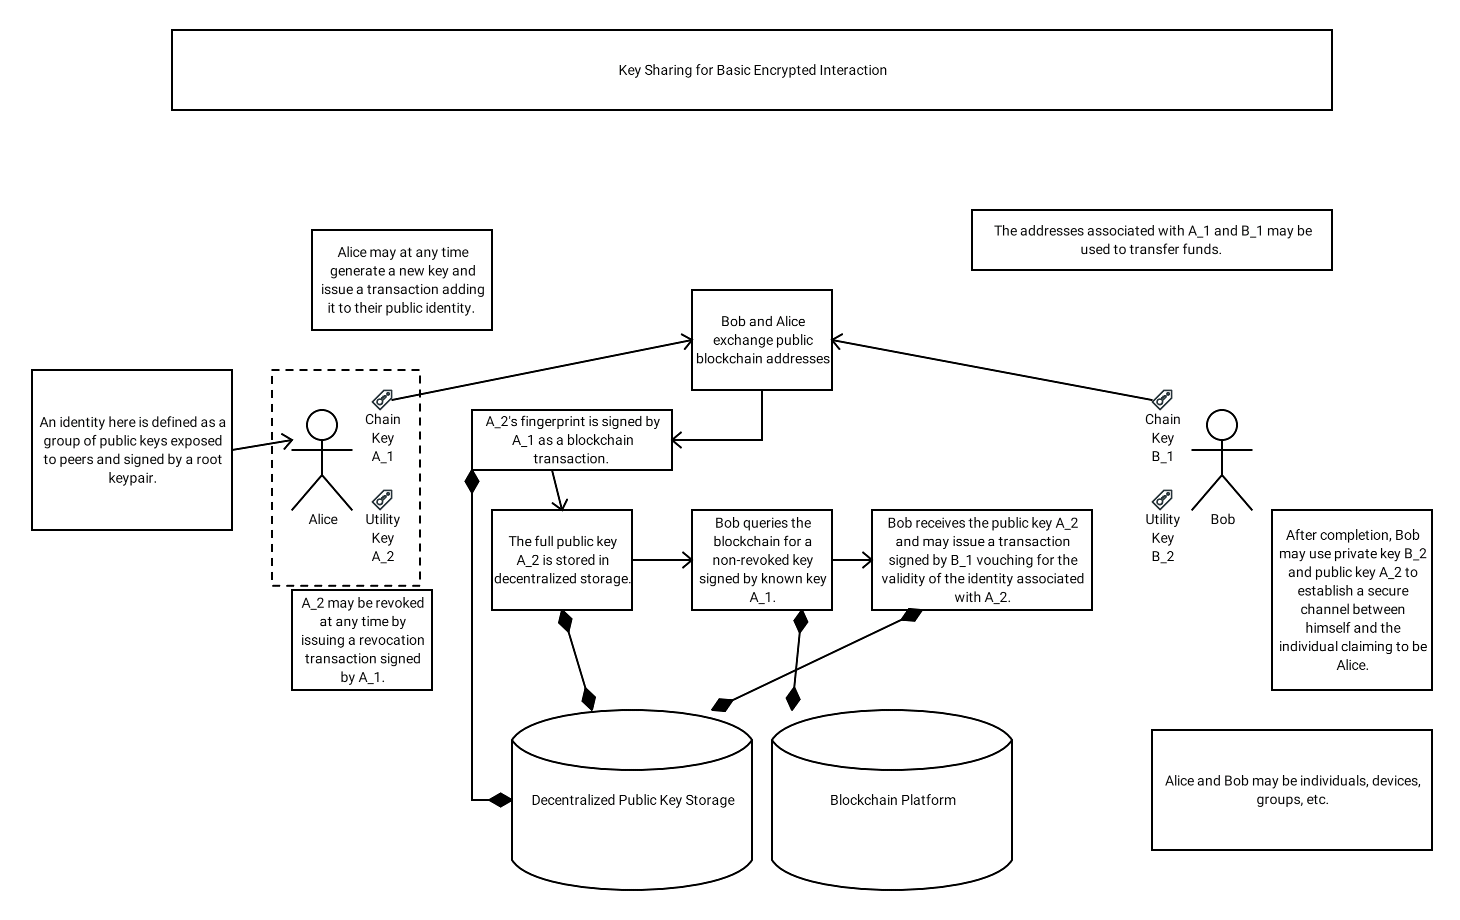
\includegraphics[width=1.2\columnwidth]{detailed-arch.png}
\caption{An outline for the key-sharing process.}
\label{scrivauto:58}
\end{figure}
\clearpage
\begin{figure}[htbp]
\centering
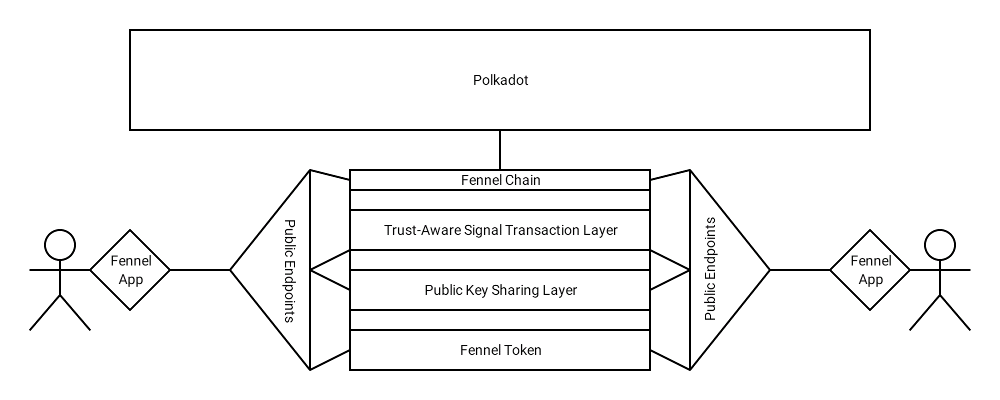
\includegraphics[width=1.2\columnwidth]{arch-overview.png}
\caption{High-level architecture.}
\label{scrivauto:59}
\end{figure}

\pagebreak
\begin{appendices}
    \printindex\pagebreak
    \printglossaries{}
    \printbibliography[heading=bibintoc]{}
\end{appendices}
\end{document}